\subsection{Newton’s Fluxions: From Geometry to Motion (1670s)}

  Isaac Newton didn’t just invent calculus: he invented a new way to think about time itself.
  
  In the \textit{Principia}, he draws a sharp distinction between two kinds of time:

  \begin{quote}
  Absolute, true, and mathematical time, of itself, and from its own nature, flows equably without relation to anything external...
  \end{quote}
  
  For Newton, time wasn’t just a coordinate. It was a cosmic river—unseen, unchanging, and universal. All motion, all change, all flux happened within this background flow. It didn’t depend on clocks or planets or observers. Time just \textit{was}, always ticking along in the background like some divine metronome.
  
  This view shaped his entire mathematical framework. The derivative—what he called the \textbf{fluxion}—wasn’t just a slope on a graph. It was a rate of change \textit{with respect to absolute time}. Every evolving quantity had a speed. Every curve had a motion. And every motion happened within the silent rhythm of Newton’s eternal clock.
  

  Where others saw geometry, Newton saw \textbf{kinematics}. Where others measured lengths, he measured \textbf{change}. And at the center of it all was time—not as an illusion, but as the most real thing in the universe.

    Before Newton, motion was geometry's unruly cousin — more art than science, more epicycle than equation. Astronomers charted paths. Mathematicians constructed curves. But few asked the deeper question: \textit{how does motion unfold through time?}

    \textbf{Kinematics} changed that.
    
    In the 17th century, a new discipline emerged — one that stripped away causes and forces and focused only on motion itself. It didn’t ask \textit{why} things moved, only \textit{how fast}, \textit{in what direction}, and \textit{how that changed over time}.

    \textbf{Key Developments:}
    

    \begin{itemize}
      \item \textbf{Galileo Galilei} studied uniformly accelerated motion and laid the groundwork for describing motion using time, distance, and velocity — even before calculus.
      \item \textbf{Isaac Newton} took this further, developing calculus as a tool for describing how quantities change — giving us acceleration, jerk, and higher derivatives as measurable realities.
      \item Kinematics became the scaffolding for Newton’s deeper theory: \textbf{dynamics}, which added force and mass into the mix.
    \end{itemize}
    
    Kinematics was the first major shift in physics to treat time as a variable rather than a stage. It formalized the idea that motion is not just spatial, but \textbf{temporal}. Every modern theory of motion — from relativity to quantum mechanics — builds on this insight.
    
    \begin{quote}
    Kinematics didn’t explain the universe.  It gave us the vocabulary to describe its dance.
    \end{quote}

To Newton, quantities were not static magnitudes, but flowing values—changing continuously with time. Instead of drawing triangles on curves, he imagined how a point moved along a curve, and how its position evolved. This shift—from shape to speed, from geometry to kinematics—transformed the mathematics of the curve into the mathematics of change itself.

He denoted this with a dot over the variable:

\[
\dot{x} = \frac{o}{\bar{o}}
\]

where:

\begin{itemize}
    \item \( o \) is an \textbf{infinitely small increment} of time.  
    \item \( \bar{o} \) is the corresponding change in \( x \).
\end{itemize}


  

Unlike his predecessors, Newton did not merely approximate motion: he embedded it into the foundations of his system. Tangents were consequences of how quantities flowed.

  Newton didn’t invent acceleration—that was Galileo, who noticed that falling objects don’t just move; they \textit{accelerate}. But Galileo stopped at observation. Newton gave it a cause—and a calculus.
  
  \textbf{Step one: Define acceleration in terms of fluxions.}  
  Using his own notation, Newton described acceleration as the \textit{fluxion of velocity}, written as:
  \[
  \dot{v}
  \]
  
  \textbf{Step two: Define momentum.}  

  He understood that the quantity of motion—what we now call momentum—was proportional to mass and velocity:
  \[
  p = m v
  \]
  
  \textbf{Step three: Relate force to the change of momentum.}  

  In the \textit{Principia}, Newton writes:

  \begin{quote}
  \textit{“The change of motion is proportional to the motive force impressed.”}
  \end{quote}

  Here, “motion” means momentum. So mathematically:

  \[
  F = \dot{p}
  \]
  
  Now, assuming mass is constant (which Newton generally did), this becomes:

  \[
  F = \dot{(mv)} = m\dot{v}
  \]
  
  \textbf{And there it is.} Not \( F = ma \), but \( F = m\dot{v} \): force as the fluxion of momentum.
  
  \textbf{Galileo saw that velocity changed with time. Newton gave that change a cause—and a law.}
  
  By linking force to motion through fluxions, Newton wasn’t just describing the world. He was explaining it—on Earth, in the heavens, and everywhere time flows.


\begin{figure}[H]
\centering
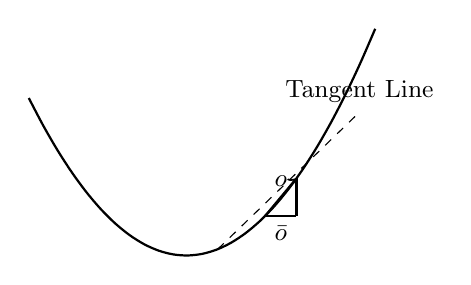
\begin{tikzpicture}[scale=2]
    % Draw the curve
    \draw[thick, domain=-1:1.2, smooth, variable=\x] plot ({\x},{\x*\x});

    % Draw infinitesimal motion
    \draw[->, thick] (0.5, 0.25) -- (0.7, 0.49) node[midway, above] {\small $o$};
    \draw[thick] (0.5, 0.25) -- (0.7, 0.25);
    \draw[thick] (0.7, 0.25) -- (0.7, 0.49);
    \node[below] at (0.6,0.25) {\small $\bar{o}$};
    
    % Draw tangent line
    \draw[dashed] (0.2, 0.04) -- (1.1, 0.91) node[above] {\small Tangent Line};

\end{tikzpicture}

\vspace{0.5em}
\caption{\small Newton's conception of calculus was rooted in geometry and motion. He imagined a point moving along a curve, where the instantaneous rate of change — the fluxion — could be represented as the ratio between an infinitesimal vertical change ($o$) and an infinitesimal horizontal change ($\bar{o}$). The resulting quantity corresponds to the slope of the tangent line at that point. This approach reflects Newton’s view of change as inherently tied to physical movement through time.}
\end{figure}




\subsubsection{Tangents and Areas} 

Building on his concept of \textit{fluxions}, Newton sought to explain the celestial mechanics that Kepler had described — particularly the Second Law: that a planet sweeps out equal areas in equal intervals of time.

But for Newton, this was more than an empirical fact — it was a geometric key.

Newton imagined a planet tracing a polygonal path around the sun, changing direction at small but finite intervals. The motion between each point was along a straight line — the tangent to the curve at that instant. A central force, acting in discrete impulses, would “bend” the path at each vertex toward the sun.

This construction allowed him to prove that if a body is always deflected toward a central point (like the Sun), then the areas swept out by its radius vector are equal over equal times.

Newton took Kepler’s geometric observation and pushed it into the realm of the infinitesimal. Instead of finite triangles, he considered the area swept out over an infinitesimal time \( \Delta t \), and then took the limit as \( \Delta t \to 0 \):

\[
\lim_{\Delta t \to 0} \frac{\Delta A}{\Delta t} = \frac{1}{2} r^2 \frac{d\theta}{dt}
\]

This quantity — the instantaneous rate of area swept — is not just a computational convenience. It’s a profound physical invariant. No matter where the planet is in its orbit—speeding up near perihelion, slowing down near aphelion—the area it sweeps out per unit of absolute time remains perfectly constant.

That constancy has teeth.

It tells us that the only possible force governing this motion must act \textit{along the radius vector}, directly between the planet and the Sun. Why? Because only a force that pulls straight inward preserves the balance of motion in just the right way to keep the area rate constant. If the force had any sideways component, it would distort the triangle—stretching or squishing the area—violating Kepler’s elegant rule.

So what Kepler described as a poetic geometry, Newton reinterpreted as a diagnostic.
\textbf{The conservation of area isn’t just a pretty fact. It’s evidence.}

It reveals that the invisible hand guiding the orbit must be a \textit{central force}—a force that always aims toward the Sun, regardless of the planet’s speed or position.

In Newton’s hands, Kepler’s Second Law transformed from a mysterious observational regularity into a tool of deduction. It became a geometric fingerprint of force direction—a testable consequence of deeper mechanics.
This was the turning point:
\textbf{Kepler gave us the pattern. Newton found the cause.}

In modern terms, we’d say that angular momentum is conserved. But in Newton’s original fluxional geometry, it was the area rate—the sweep of triangles over time—that carried the truth.
And that truth pointed like an arrow straight to the Sun.

\begin{figure}[H]
\centering
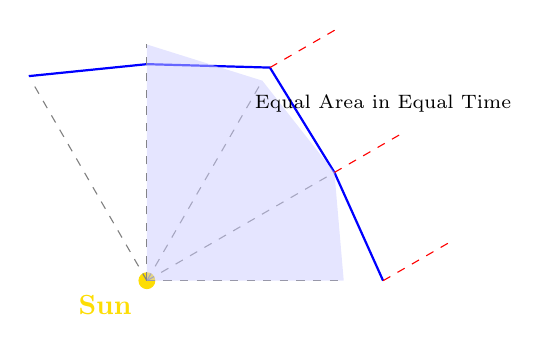
\begin{tikzpicture}[scale=2.5]

  % Sun at origin
  \filldraw[yellow!80!orange] (0,0) circle (0.04) node[below left=2pt] {\textbf{Sun}};

  % Orbit path (approx polygonal)
  \draw[thick, blue] (0:1.2) -- (30:1.1) -- (60:1.25) -- (90:1.1) -- (120:1.2);

  % Radius vectors
  \foreach \a in {0,30,60,90,120} {
    \draw[gray, dashed] (0,0) -- (\a:{1 + 0.2*sin(\a)});
  }

  % Tangents
  \draw[dashed, red] (0:1.2) -- ++(30:0.4);
  \draw[dashed, red] (30:1.1) -- ++(30:0.4);
  \draw[dashed, red] (60:1.25) -- ++(30:0.4);

  % Area sectors (for visual)
  \foreach \a/\b in {0/30, 30/60, 60/90} {
    \fill[blue!20, opacity=0.5] (0,0) -- (\a:{1 + 0.2*sin(\a)}) -- (\b:{1 + 0.2*sin(\b)}) -- cycle;
  }

  \node at (1.2, 0.9) {\scriptsize Equal Area in Equal Time};

\end{tikzpicture}
\caption{Newton’s polygonal construction: a planet moving in equal time steps traces out equal areas. Each segment approximates a tangent; each deflection represents a central force impulse. In the limit of infinitely small time steps, the motion becomes smooth and the area swept per unit time becomes \( \frac{1}{2} r^2 \frac{d\theta}{dt} \), a constant.}
\end{figure}

\subsubsection{From Area to Force} 

In Proposition I of the \textit{Principia}, Newton proved:  

\textit{“A body under a centripetal force sweeps out equal areas in equal times.”}

The converse is also true: if equal areas are swept in equal time, then the force must point toward the center. The notion of “force” is geometric. It’s the repeated deflection of the tangent line by an inward-pulling agent.

\subsubsection{From Fluxions to Gravity.} 

Once Newton had this geometric foundation, he began to explore the nature of the force itself.

In Proposition XI of the \textit{Principia}, he showed that if a planet’s orbit is an ellipse and the force is centripetal, then the force must be inversely proportional to the square of the distance:

\[
F \propto \frac{1}{r^2}
\]

To derive this, Newton analyzed how the velocity (the fluxion of position) changes along the curve. Using geometry and proportions, he established that the acceleration required to maintain the elliptical orbit — which he related to curvature and tangents — must obey this inverse-square law.

This, combined with Kepler’s laws, gave the world its first universal law of gravitation.

\subsubsection{Tangents as the Language of Force.} 

In Newton’s hands, the tangent was more than a line — it was a law. The fluxion $\dot{x}$ described the direction and speed of a moving point; the change of the tangent described acceleration; and acceleration, in Newton’s system, was nothing other than force.

\[
\text{Fluxion} \rightarrow \text{Tangent} \rightarrow \text{Change of Tangent} \rightarrow \text{Force}
\]

This wasn’t just a mathematical trick — it was a physical revolution.


\begin{tcolorbox}[colback=gray!5!white, colframe=black, title=\textbf{Historical Sidebar: Newton’s Fluxions and the Geometry of Instantaneous Motion}, fonttitle=\bfseries, arc=1.5mm, boxrule=0.4pt]

  When Isaac Newton analyzed planetary motion, he built directly on \textbf{Kepler’s Second Law}—that a planet sweeps out \textit{equal areas in equal times}. But where Kepler reasoned in finite steps, Newton introduced the mathematics of the \textit{instant}.
  
  Using his method of \textbf{fluxions}, Newton reinterpreted Kepler’s geometric insight in terms of \textit{momentary motion}. He considered an infinitely small duration of time and the triangular area swept out in that instant.
  
  \vspace{0.5em}
  If a planet is at distance \( r \) from the center and moving with angular fluxion \( \dot{\theta} \), then the rate at which area is swept out—the \textit{fluxion of area}—is:
  
  \[
  \dot{A} = \frac{1}{2} r^2 \dot{\theta}
  \]
  
  This quantity, \( \dot{A} \), remains constant under a centripetal force. Newton took this as more than a computational result—it was a geometric truth in motion.
  
  \vspace{0.5em}
  From this, he concluded that the governing force must be \textbf{directed toward the center}, for only such a force maintains the constancy of \( \dot{A} \).
  
  \[
  \text{Constancy of } \dot{A} \quad \Rightarrow \quad \text{Force directed along the radius}
  \]
  
  Newton thus extracted a law of force from a law of area—not through algebra, but through the geometry of instantaneous change. This was the turning point where discrete planetary geometry became continuous mechanics.
  
\end{tcolorbox}
  